%\appendix
\chapter{Fully Probabilistic Galaxy Cluster Membership Determination}
\label{chapter:ProbMembDetappendix}

\section{Method}
This membership determination method is rooted in the desire to treat both spectroscopic and photometric redshift samples in a consistent manner. 
This method slightly favors minimizing the Poisson noise while still trying to address the systematic contamination error. 
The basic approach is to assign a weight to each galaxy based on its probability of being a cluster member.
This weight is defined as the inner product of the redshift probability density function (PDF) of a galaxy $p_i(z)$ and the redshift velocity dispersion ($\sigma_{\rm vdisp}$assumed to be Gaussian) of the cluster at redshift $z_{\rm cluster}$,
\begin{equation}
w_i = \int_{0}^{\infty} p_i(z) \frac{1}{\sigma_{\rm vdisp}\sqrt{2\pi}}e^{\frac{-(z-z_{\rm cluster})^2}{2\sigma_{\rm vdisp}^2}}\mathrm{d}z.
\label{equation:genericz_weight}
\end{equation}
Since the redshift uncertainty of a spectroscopically observed galaxy with $z_{\rm spec_{i}}$ is $\ll \sigma_{\rm vdisp} (1+z_{\rm cluster}) c^{-1}$, its redshift PDF can be treated as a delta-function and Equation \ref{equation:genericz_weight} reduces to
\begin{equation}
w_i = \frac{1}{\sigma_{\rm vdisp}\sqrt{2\pi}}e^{\frac{-(z_{\rm spec_{i}}-z_{\rm cluster})^2}{2\sigma_{\rm vdisp}^2}}.
\end{equation}\label{equation:specz_weight}
Under the assumption of Gaussian photometric redshift errors\footnote{In reality there are a small fraction of galaxies, known as catastrophic outliers, that violate this assumption \citep[see][for a detailed discussion]{Schmidt:2013ig}. For the case of DLS photometric redshifts the outlier fraction is $\lesssim$5\%, thus they should not significantly violate the assumptions of this method.} ($\sigma_{\rm z-phot_{i}} \approx \bar{\sigma}(1+z_{\rm phot_{i}})$; $\bar{\sigma}$=0.07 for the Musket Ball Cluster) Equation \ref{equation:genericz_weight} takes the form
\begin{equation}
w_i = \int_{0}^{\infty} \frac{1}{\sigma_{\rm z-phot_{i}}\sqrt{2\pi}}e^{\frac{-(z-z_{\rm phot_{i}})^2}{2\sigma_{\rm z-phot_{i}}^2}} \frac{1}{\sigma_{\rm vdisp}\sqrt{2\pi}}e^{\frac{-(z-z_{\rm cluster})^2}{2\sigma_{\rm vdisp}^2}}\mathrm{d}z.
\label{equation:photoz_weight}
\end{equation}

When estimating the galaxy centroid these weights are simply used in conjunction with Equation \ref{equation:WeightedCentroid}.
The bootstrap realizations used in the centroid uncertainty estimate are handled in a slightly different but equivalent manner.
Using these weights we form a cumulative normalized weight distribution for all the galaxies with $R<24$ and within a 9' by 9' region surrounding the Musket Ball Cluster (see Figure \ref{figure:NormWeightDist}).
During the bootstrap sampling process a random number between 0 and 1 is drawn from a uniform distribution, where this random number intersects the weight distribution determines the randomly selected galaxy.
Beyond this weighted draw with replacement the bootstrap uncertainty analysis is standard in all regards.

\begin{figure}
\centering
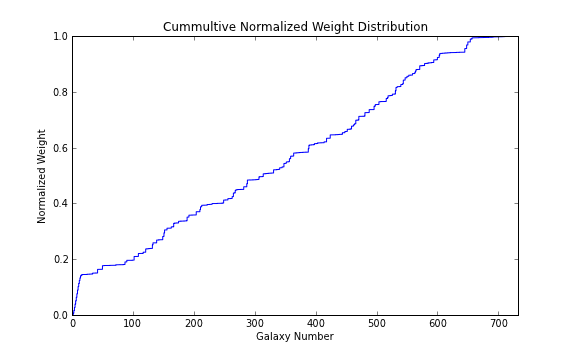
\includegraphics[width=4in]{Chapter4/AnalysisFiles/cumnormwghtdist.png}
\caption[Probabilistic scheme; cumulative normalized weight distribution for galaxies being in the Musket Ball Cluster.]{
The resulting cumulative weight distribution for all the galaxies with $R<24$ and within a 9' by 9' region surrounding the Musket Ball Cluster.
This distribution is used to perform a weighted random draw of cluster galaxies (e.g. the green distribution of Figure \ref{figure:ProbWeightDist}) for the galaxy centroid bootstrap analysis.
This distribution is determined by Equations \ref{equation:specz_weight} and \ref{equation:photoz_weight}.
During the bootstrap sampling process a random number between 0 and 1 is drawn from a uniform distribution, where this random number intersects the weight distribution determines the randomly selected galaxy.
Note that the catalog is sorted such that the spectroscopic members are first, thus the noticeably steeper slope for the early galaxy numbers.
}
\label{figure:NormWeightDist}
\end{figure}

Comparing the galaxy redshift distribution of a random bootstrap realization with the redshift distribution of the parent population (Figure \ref{figure:ProbWeightDist}) it is apparent that the fully probabilistic membership determination scheme still includes a large number of galaxies with photometric redshift estimates well outside the cluster redshift velocity dispersion ($z_{\rm cluster}\pm\sigma_{\rm vdisp} (1+z_{\rm cluster}) c^{-1} \approx 0.53\pm0.004$).
The reason for this is simply that the photometric redshift uncertainties are so large compared to all other pertinent redshift scales.
Thus, galaxies that have the exact same photometric redshift as the cluster are not weighted dramatically more than galaxies with photometric redshift estimates well in front of or behind the cluster.
Take for example two photometric redshift galaxies, one at the cluster redshift ($z=0.53$) and one well behind the cluster at $z_{\rm phot}=0.79$.
According to Equation \ref{equation:photoz_weight} the galaxy with $z_{\rm phot}=0.53$ will have a weight of 3.7 while the galaxy with $z_{\rm phot}=0.79$ will have a weight of 0.37.
Since even in this small projected region around the Musket Ball Cluster the number of fore/background galaxies outnumber the cluster members, this probabilistic weighting scheme will always result in a significant amount of contamination.
This is why \citet{George:2011kv} base their probability of cluster membership both on the expected distribution of the cluster members as well as the field.
Such a method is worth considering for future work but is currently beyond the scope of this dissertation.
Instead we use an empirically based method to determine our weighting scheme for cluster membership (see \S\ref{section:EmpiricalWeightScheme}). 


\begin{figure}
\centering
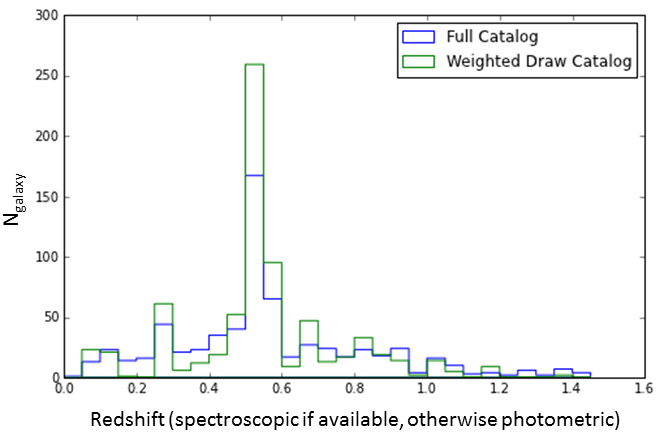
\includegraphics[width=4in]{Chapter4/AnalysisFiles/zdist_randomweightdraw_reformat.png}
\caption[Comparison of parent galaxy redshift distribution with weighted random draw distribution.]{
The redshift (spectroscopic if available, otherwise photometric) distribution of all the galaxies in a 9'$\times$9' area surrounding the Musket Ball Cluster with $R<$24 (blue); and a single bootstrap sample (green) drawn from the fully probabilistic weighted distribution (Figure \ref{figure:NormWeightDist}).
While the probabilistic scheme does work to increase the number of galaxies selected at the cluster redshift ($z=0.53$) it still selects a disproportionate number of galaxies with photometric redshifts outside of the cluster redshift; see that in Figure \ref{figure:photzVSspecz} only 1 galaxy of our spectroscopic survey sample with $z_{\rm phot}>$0.7 is actually at the cluster redshift and only 1 galaxy with $z_{\rm phot}<$0.43 is at the cluster redshift.
}
\label{figure:ProbWeightDist}
\end{figure}

